\documentclass{article}
\usepackage[utf8]{inputenc}
\usepackage{graphicx}
\begin{document}
\title{Introduction to \LaTeX{}}
\author{Author Name}
\maketitle
\tableofcontents
\begin{abstract}
The abstract---the façade of your article---goes here.
\end{abstract}
\section{Introduction}
Here's the text of your introduction.
\begin{equation}
  \label{simple_equation}
  \alpha = \sqrt{ \beta }
\end{equation}
\subsection{Subsection Heading}
Write your subsection text here.
\begin{figure}
  \centering
  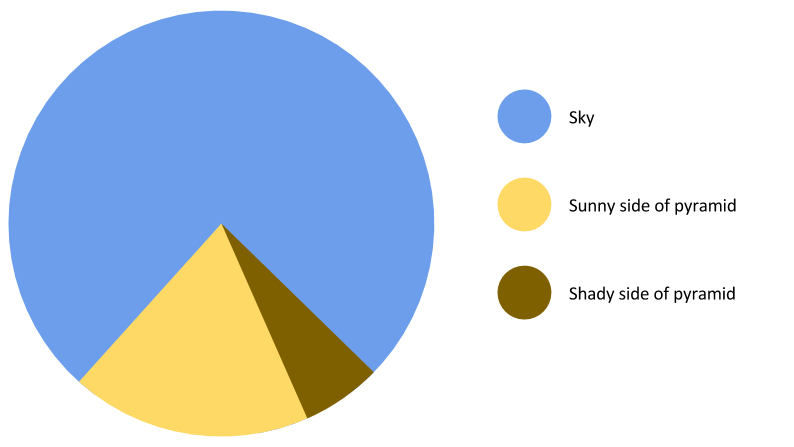
\includegraphics[width=3.0in]{images/figure}
  \caption{Simulation Results}
  \label{simulation_figure}
\end{figure}
\section{Conclusion}
Write your conclusion here.
\end{document}
